% F01: Histogram of ISI composite scores
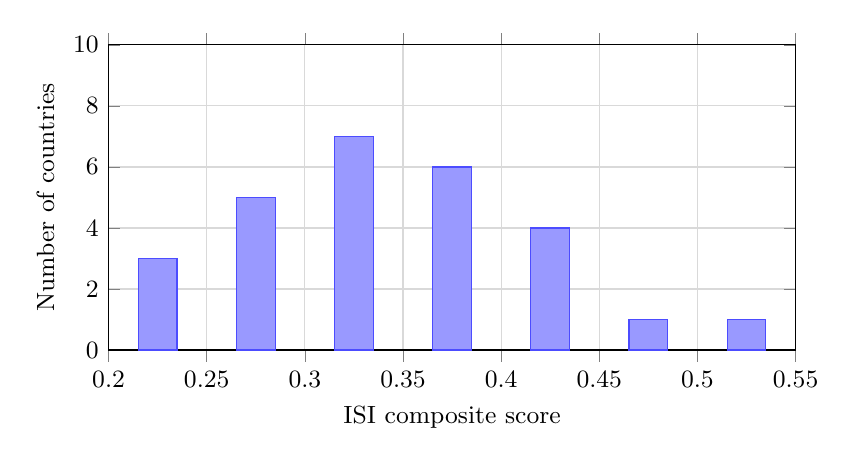
\begin{tikzpicture}
\begin{axis}[
  ybar,
  bar width=14pt,
  width=0.85\textwidth,
  height=0.45\textwidth,
  xlabel={ISI composite score},
  ylabel={Number of countries},
  xmin=0.20, xmax=0.55,
  ymin=0, ymax=10,
  xtick={0.20,0.25,0.30,0.35,0.40,0.45,0.50,0.55},
  ytick={0,2,4,6,8,10},
  grid=major,
  grid style={gray!30},
  tick label style={font=\small},
  label style={font=\small},
]
% Bin edges: 0.20-0.25, 0.25-0.30, 0.30-0.35, 0.35-0.40, 0.40-0.45, 0.45-0.50, 0.50-0.55
% Counts from data: [3, 5, 7, 6, 4, 1, 1]
\addplot[fill=blue!40, draw=blue!70] coordinates {
  (0.225, 3)
  (0.275, 5)
  (0.325, 7)
  (0.375, 6)
  (0.425, 4)
  (0.475, 1)
  (0.525, 1)
};
\end{axis}
\end{tikzpicture}
